\section{Overview and experimental design}
\label{research-design-and-methodology:overview-and-experimental-design}

This chapter sets out the plan that the remainder of the thesis carries out: what is varied, what is held constant, how each outcome is measured in principle, and how the resulting samples are analyzed. The design answers two questions. The first asks how the cloud-native combination of GeoParquet and DuckDB compares with the traditional alternatives, PostGIS and Shapefile, in wall-clock query time, network transfer, and operational cost, evaluated across spatial intersection predicates, distance-based nearest-neighbor search, and bounding-box range filtering on Norwegian building data at small and large dataset tiers. The second asks, for a national-scale spatial join on the same data, how broadcast-join and partitioned-join execution strategies on Apache Sedona compare against single-node PostGIS and DuckDB in wall-clock time, scaling behavior, network transfer, and operational cost across the same tiers.

Three methodological commitments separate this design from the prior benchmarks reviewed in Chapter~\ref{ch:related-work}. First, end-to-end network transfer is treated as a primary outcome and measured directly at the client, rather than inferred from format internals or omitted. Second, cloud-native and traditional configurations are compared on an identical workload using identical data, so that any observed difference is attributable to the format-and-engine pairing rather than to a divergence in inputs. Third, single-node and distributed engines are placed within a single comparison framework and reported on the same axes of time, transferred bytes, and cost, which lets the question of when distribution repays its coordination overhead be answered against a single-node reference rather than asserted. That a distributed engine outperforms a single-node one only once the dataset or computation is large enough to justify its coordination cost is established in Section~\ref{background:cloud-native-data-architecture:distributed-and-non-distributed-computation} and is the premise that the third commitment operationalizes.

These commitments resolve into four design cells formed by crossing two axes: cloud-native versus traditional and single-node versus distributed. The cloud-native single-node cell pairs DuckDB with GeoParquet; the traditional single-node cell uses PostGIS and reads Shapefiles locally; the cloud-native distributed cell uses Sedona over GeoParquet. The cells are stated here at the level of format-and-engine pairings, the unit on which the comparison turns, and are laid out in Figure~\ref{fig:design-space}. Their concrete realization, including the compute platform, storage layout, and engine versions, is an implementation detail and is described in Chapter~\ref{ch:system-architecture-and-implementation}.

\begin{figure}[H]
    \centering
    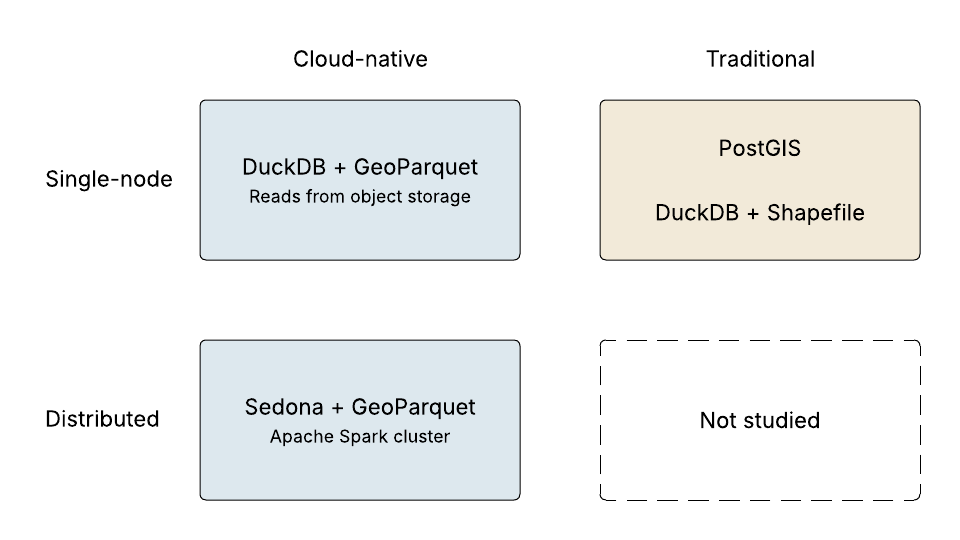
\includegraphics[width=0.85\textwidth]{Chapters/04-research-design-and-methodology/sub-chapters/figures/04-design-space.png}
    \caption[The four design cells of the experimental design]{The experimental design space, formed by crossing the cloud-native/traditional axis with the single-node/distributed axis. Three cells are populated by format-and-engine configurations; the traditional distributed cell is left unstudied, as no traditional format targets a distributed run-time in this comparison.}
    \label{fig:design-space}
\end{figure}

\subsection{Factors and levels}
\label{research-design-and-methodology:overview-and-experimental-design:factors-and-levels}

The two research questions differ in several respects. \acrshort{rq}1 varies a single factor, the configuration, across four levels: DuckDB over GeoParquet, PostGIS, DuckDB over Shapefile, and Sedona over GeoParquet. \acrshort{rq}2 varies the worker count of the distributed engine across five levels, from 2 to 16 nodes, to trace how the spatial join scales with increasing parallelism. Both questions treat the workload as a secondary factor, with the query patterns and their definitions given in Section~\ref{research-design-and-methodology:workloads}. To isolate these factors, the dataset, the regions it covers, the sizing of the client compute, the client process that issues each query, and the access protocol are held constant across every level, so that a difference in an outcome reflects the factor under test and not a difference in inputs or in the measurement apparatus. Table~\ref{tab:methodology:factors} summarizes the factors, their levels, and the question each addresses.

\begin{table}[H]
    \centering
    \begin{tabular}{@{}l l p{6.5cm} l@{}}
        \toprule
        \textbf{Factor} & \textbf{Role} & \textbf{Levels} & \textbf{RQ} \\
        \midrule
        Configuration & Varied      & DuckDB + GeoParquet, PostGIS, DuckDB + Shapefile, Sedona + GeoParquet & \acrshort{rq}1 \\
        Worker count  & Varied      & 2, 4, 8, 12, 16 & \acrshort{rq}2 \\
        Workload      & Varied      & See Section~\ref{research-design-and-methodology:workloads} & \acrshort{rq}1, \acrshort{rq}2 \\
        \midrule
        Dataset, regions & Constant & Identical inputs across every level & --- \\
        Client compute   & Constant & Same instance sizing and process & --- \\
        Access protocol  & Constant & Same protocol across configurations & --- \\
        \bottomrule
    \end{tabular}
    \caption[Experimental factors and controls]{Factors varied in the experiment, the controls held constant across all levels, and the research question each factor addresses.}
    \label{tab:methodology:factors}
\end{table}

\subsection{Replication and randomization}
\label{research-design-and-methodology:overview-and-experimental-design:replication-and-randomization}

Each query is executed as a sequence of $N$ warmup iterations followed by $M$ timed iterations, with the warmup results discarded. Warmup primes caches and connection state so that the timed iterations measure an engine in steady operation rather than its cold start. The count $M$ is calibrated per workload, with cheap high-frequency queries given many iterations and the expensive national-scale join given few, so that every workload yields a sample large enough to characterize its distribution without spending run-time on iterations that add no information.

Within each benchmark run, the execution order of the experiments is randomized using a seeded random number generator, and the seed is reused across runs to ensure reproducibility. Randomizing the order of test and control measurements on the same instance is a practice shown to reliably detect small slowdowns under cloud variability \parencite{laaber2019_software_microbenchmarking_cloud}. Configurations that are compared on the same workload are additionally paired and launched concurrently on identically provisioned client instances, so that the two members of a comparison share the same short-term conditions and the time-of-day variance between them is reduced rather than left to vary run by run \parencite{laaber2019_software_microbenchmarking_cloud}. The distributed configuration is the one exception to the warmup discipline: because each of its runs provisions a fresh cluster, warmup iterations would multiply provisioning cost without priming a persistent engine, so they are omitted, and the resulting variance is treated separately in Section~\ref{research-design-and-methodology:statistical-analysis}. The mechanisms that realize this protocol, the orchestration, the container sizing, and the cluster lifecycle, are deferred to Chapter~\ref{ch:system-architecture-and-implementation}.